\documentclass[12pt, compress, aspectratio=1610]{beamer}

\usetheme{pl}

\usepackage{longtable}
\usepackage{booktabs}
\usepackage{minted}
\usepackage{listings}
\usepackage{color}
\usepackage{fancyvrb}
\newcommand{\VerbBar}{|}
\newcommand{\VERB}{\Verb[commandchars=\\\{\}]}
\DefineVerbatimEnvironment{Highlighting}{Verbatim}{commandchars=\\\{\},fontsize=\small}
% Add ',fontsize=\small' for more characters per line
\usepackage[framemethod=tikz]{mdframed}
\definecolor{shadecolor}{HTML}{EEEEEE}
\mdfsetup{
  backgroundcolor=shadecolor,
  linecolor=shadecolor,
  innerleftmargin=5pt,
  innerrightmargin=5pt,
  leftmargin=-5pt,
  rightmargin=-5pt,
  roundcorner=3pt
}
\newenvironment{Shaded}{\begin{mdframed}}{\end{mdframed}}
\newcommand{\KeywordTok}[1]{\textcolor[rgb]{0.26,0.66,0.93}{\textbf{{#1}}}}
\newcommand{\DataTypeTok}[1]{\textcolor[rgb]{0.74,0.68,0.62}{\underline{{#1}}}}
\newcommand{\DecValTok}[1]{\textcolor[HTML]{558B2F}{{#1}}}
\newcommand{\BaseNTok}[1]{\textcolor[HTML]{558B2F}{{#1}}}
\newcommand{\FloatTok}[1]{\textcolor[HTML]{558B2F}{{#1}}}
\newcommand{\ConstantTok}[1]{\textcolor[rgb]{0.74,0.68,0.62}{{#1}}}
\newcommand{\CharTok}[1]{\textcolor[HTML]{7E57C2}{{#1}}}
\newcommand{\SpecialCharTok}[1]{\textcolor[HTML]{7E57C2}{{#1}}}
\newcommand{\StringTok}[1]{\textcolor[HTML]{7E57C2}{{#1}}}
\newcommand{\VerbatimStringTok}[1]{\textcolor[HTML]{7E57C2}{{#1}}}
\newcommand{\SpecialStringTok}[1]{\textcolor[HTML]{7E57C2}{{#1}}}
\newcommand{\ImportTok}[1]{\textcolor[rgb]{0.74,0.68,0.62}{{#1}}}
\newcommand{\CommentTok}[1]{\textcolor[HTML]{546E7A}{\textit{{#1}}}}
\newcommand{\DocumentationTok}[1]{\textcolor[HTML]{BCAAA4}{\textit{{#1}}}}
\newcommand{\AnnotationTok}[1]{\textcolor[HTML]{BCAAA4}{\textbf{\textit{{#1}}}}}
\newcommand{\CommentVarTok}[1]{\textcolor[rgb]{0.74,0.68,0.62}{{#1}}}
\newcommand{\OtherTok}[1]{\textcolor[rgb]{0.74,0.68,0.62}{{#1}}}
\newcommand{\FunctionTok}[1]{\textcolor[HTML]{26A69A}{\textbf{{#1}}}}
\newcommand{\VariableTok}[1]{\textcolor[rgb]{0.74,0.68,0.62}{{#1}}}
\newcommand{\ControlFlowTok}[1]{\textcolor[rgb]{0.26,0.66,0.93}{\textbf{{#1}}}}
\newcommand{\OperatorTok}[1]{\textcolor[rgb]{0.74,0.68,0.62}{{#1}}}
\newcommand{\BuiltInTok}[1]{\textcolor[HTML]{42A5F5}{{#1}}}
\newcommand{\ExtensionTok}[1]{\textcolor[rgb]{0.74,0.68,0.62}{{#1}}}
\newcommand{\PreprocessorTok}[1]{\textcolor[rgb]{0.74,0.68,0.62}{\textbf{{#1}}}}
\newcommand{\AttributeTok}[1]{\textcolor[rgb]{0.74,0.68,0.62}{{#1}}}
\newcommand{\RegionMarkerTok}[1]{\textcolor[rgb]{0.74,0.68,0.62}{{#1}}}
\newcommand{\InformationTok}[1]{\textcolor[rgb]{0.00,0.40,1.00}{\textbf{\textit{{#1}}}}}
\newcommand{\WarningTok}[1]{\textcolor[HTML]{FF6E40}{\textbf{{#1}}}}
\newcommand{\AlertTok}[1]{\textcolor[HTML]{FF3D00}{{#1}}}
\newcommand{\ErrorTok}[1]{\textcolor[HTML]{DD2C00}{\textbf{{#1}}}}
\newcommand{\NormalTok}[1]{\textcolor[HTML]{212121}{{#1}}}

% For adding citations/credits to slides
\newcommand{\btVFill}{\vskip0pt plus 1filll}
\newcommand{\credit}[1]{\btVFill\par\hfill \footnotesize ~#1}

\providecommand{\tightlist}{%
  \setlength{\itemsep}{0pt}\setlength{\parskip}{0pt}}

\let\OldTexttt\texttt
\renewcommand{\texttt}[1]{\OldTexttt{\color{codecolor}#1}}

\makeatletter
\def\maxwidth{\ifdim\Gin@nat@width>\linewidth\linewidth\else\Gin@nat@width\fi}
\makeatother

\usepgfplotslibrary{dateplot}

\newcommand{\begincols}{\begin{columns}}
\newcommand{\stopcols}{\end{columns}}
\newcommand{\roundpicture}[2]{%
\tikz\node[circle,
          text=white,
          minimum width=4cm,
          minimum height=4cm,
          path picture={
              \node at (path picture bounding box.center){
                  \includegraphics[width=4cm]{#1}
              };
          }]{#2};
}
\newcommand{\plain}[1]{%
\begin{picture}(0,0)
  \put(-28.5,-175){%
      \pgfuseimage{titlebackground}
  }
  \put(0,-145){%
      \begin{minipage}[b][4.5cm][t]{0.7\textwidth}
          \Large
          #1
      \end{minipage}
  }
\end{picture}
}

\title{Spatiotemporal forecasting of plant populations and a proposal to
partition forecast uncertainty}
\subtitle{}
\date{October 12, 2018}
\author{Andrew Tredennick}
\institute{University of Georgia}

\begin{document}

\maketitle

\begin{frame}{%
\protect\hypertarget{forecasting}{%
Forecasting}}

Skillfull forecasts are in high demand because the world is changing
fast.

\begin{enumerate}
[1.]
\tightlist
\item
  Responses to global climate change
\item
  Species invasions
\item
  Emergence and spread of infectious diseases
\end{enumerate}

\end{frame}

\begin{frame}{%
\protect\hypertarget{forecasting-1}{%
Forecasting}}

Skillfull forecasts are in high demand because the world is changing
fast.

\begin{enumerate}
[1.]
\tightlist
\item
  \alert{Responses to global climate change}
\item
  Species invasions
\item
  Emergence and spread of infectious diseases
\end{enumerate}

\end{frame}

\hypertarget{plant-population-forecasts}{%
\section{Plant population forecasts}\label{plant-population-forecasts}}

\begin{frame}{%
\protect\hypertarget{collaborators}{%
Collaborators}}

\(\phantom{testtestttttt}\) Peter Adler (USU) \hspace{9em} Mevin Hooten
(CSU)

\(\phantom{testtest}\) \roundpicture{images/peter.jpg}{} \hspace{5em}
\roundpicture{images/mevin.jpg}{}

\end{frame}

\begin{frame}{%
\protect\hypertarget{what-land-managers-want}{%
What land managers want}}

\centering

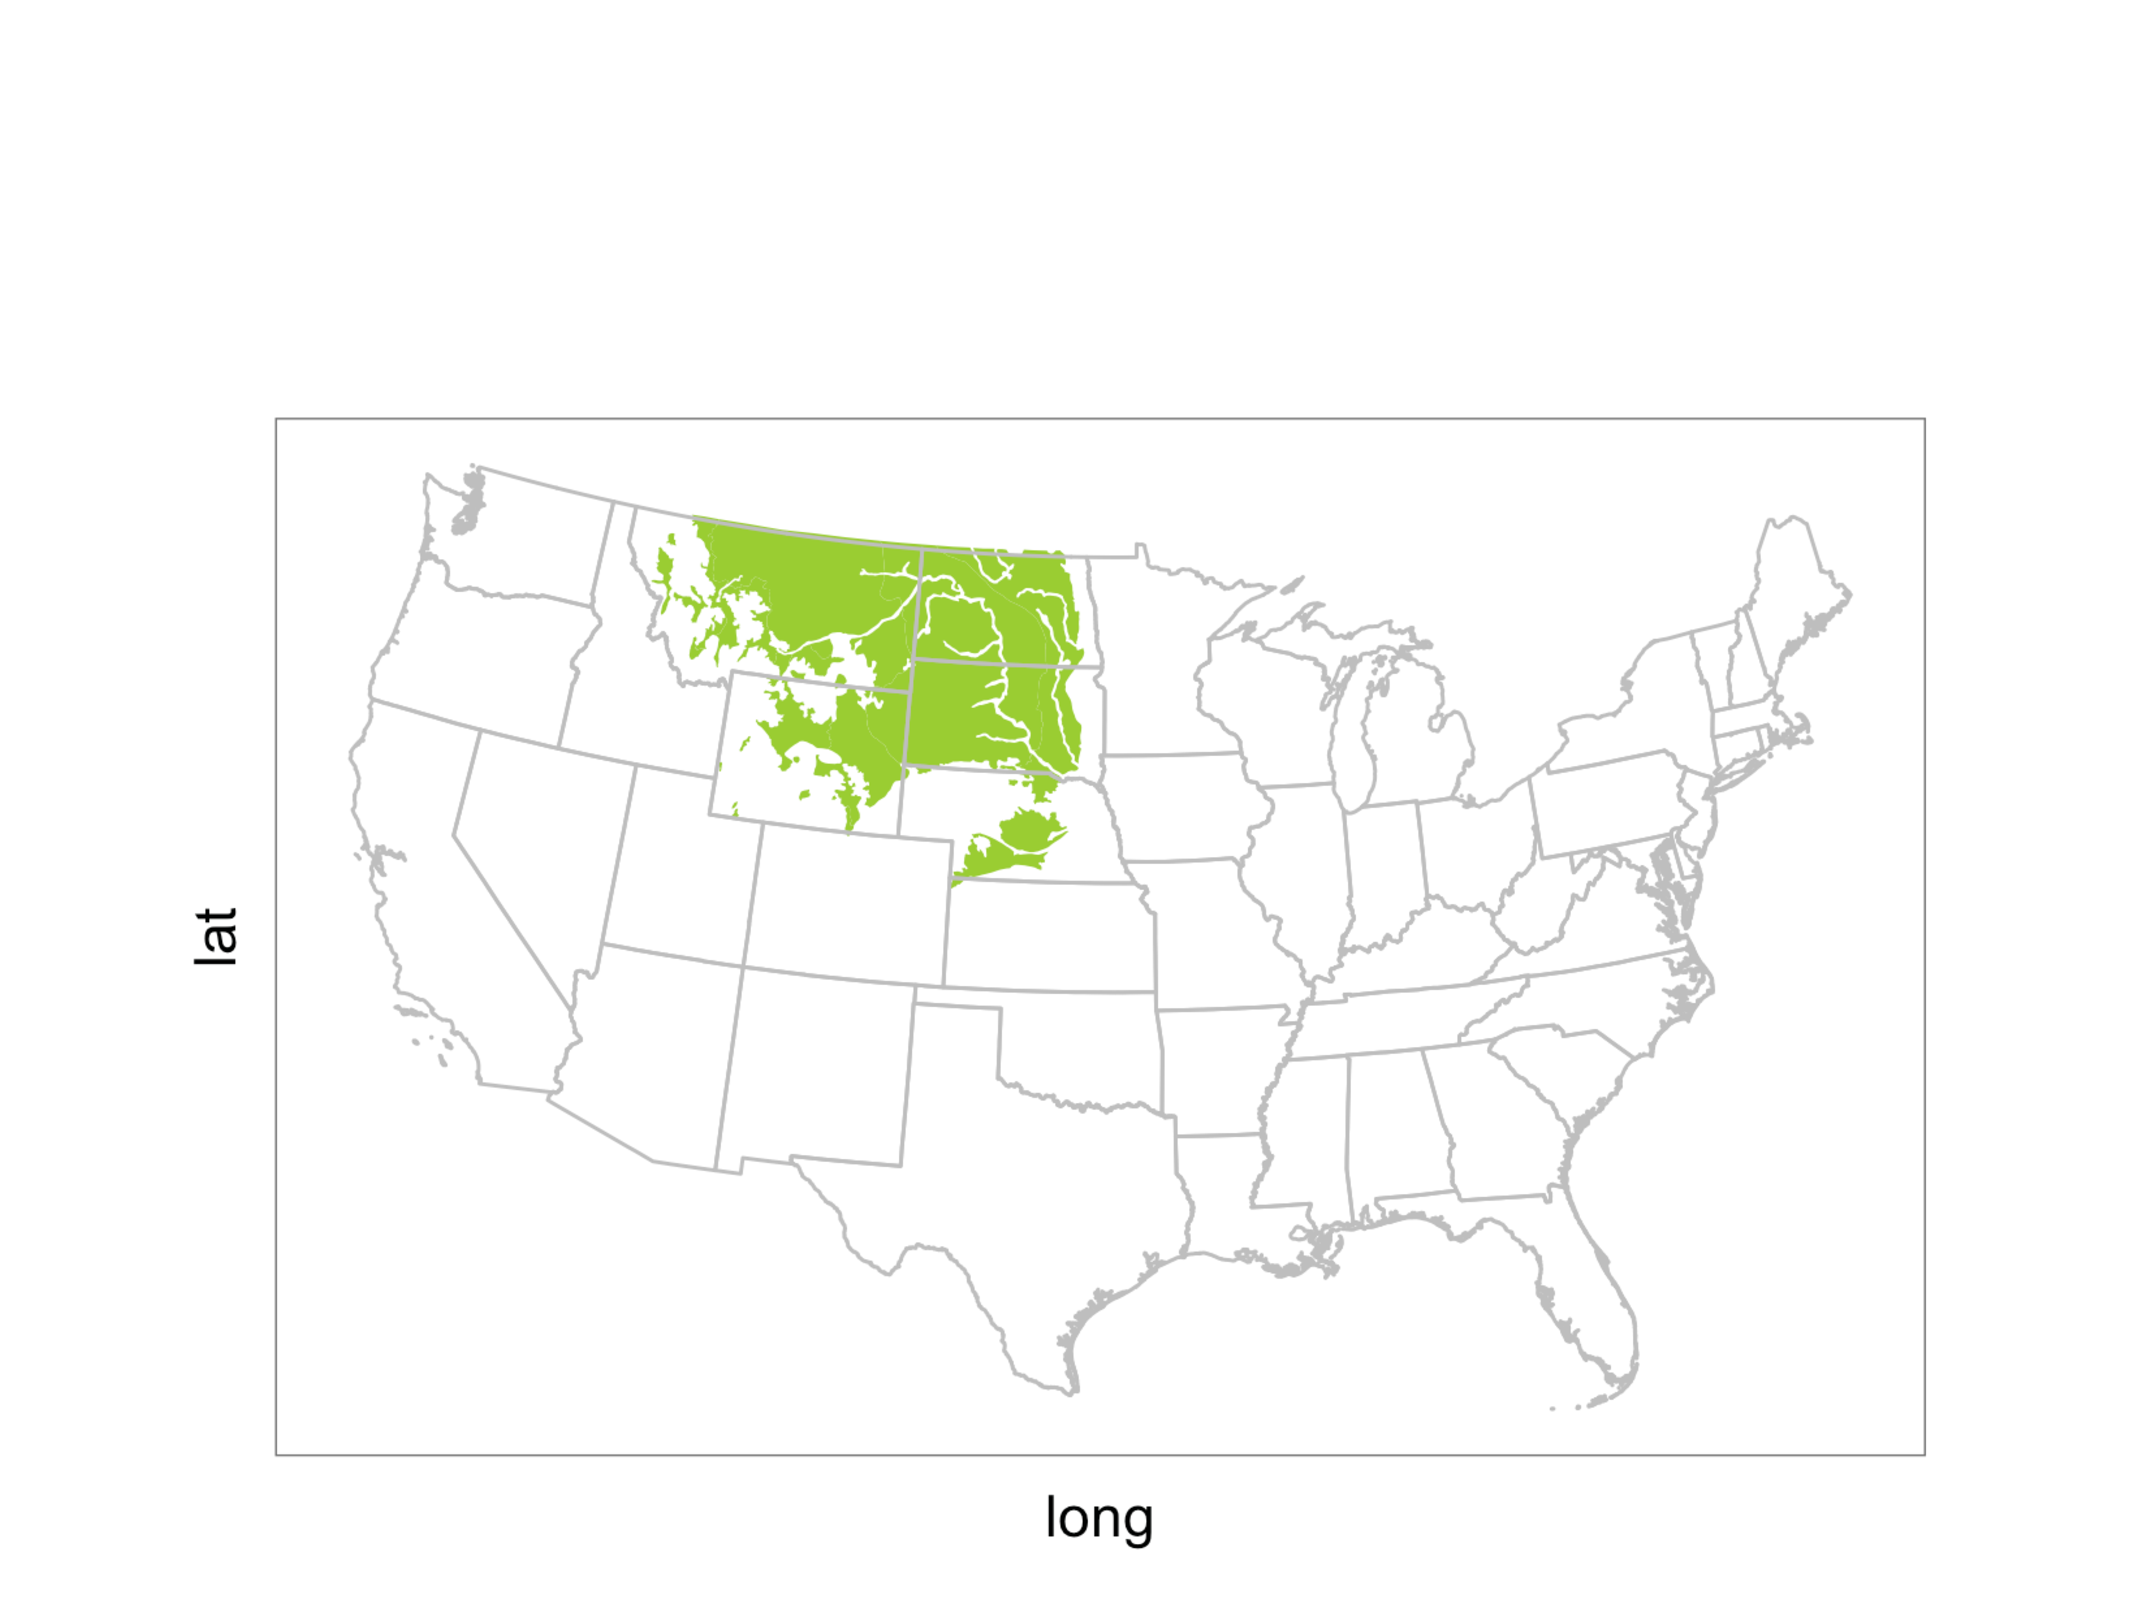
\includegraphics[height=2.7in]{./figures/managers_want.pdf}

\end{frame}

\begin{frame}{%
\protect\hypertarget{what-land-managers-get}{%
What land managers get}}

\centering

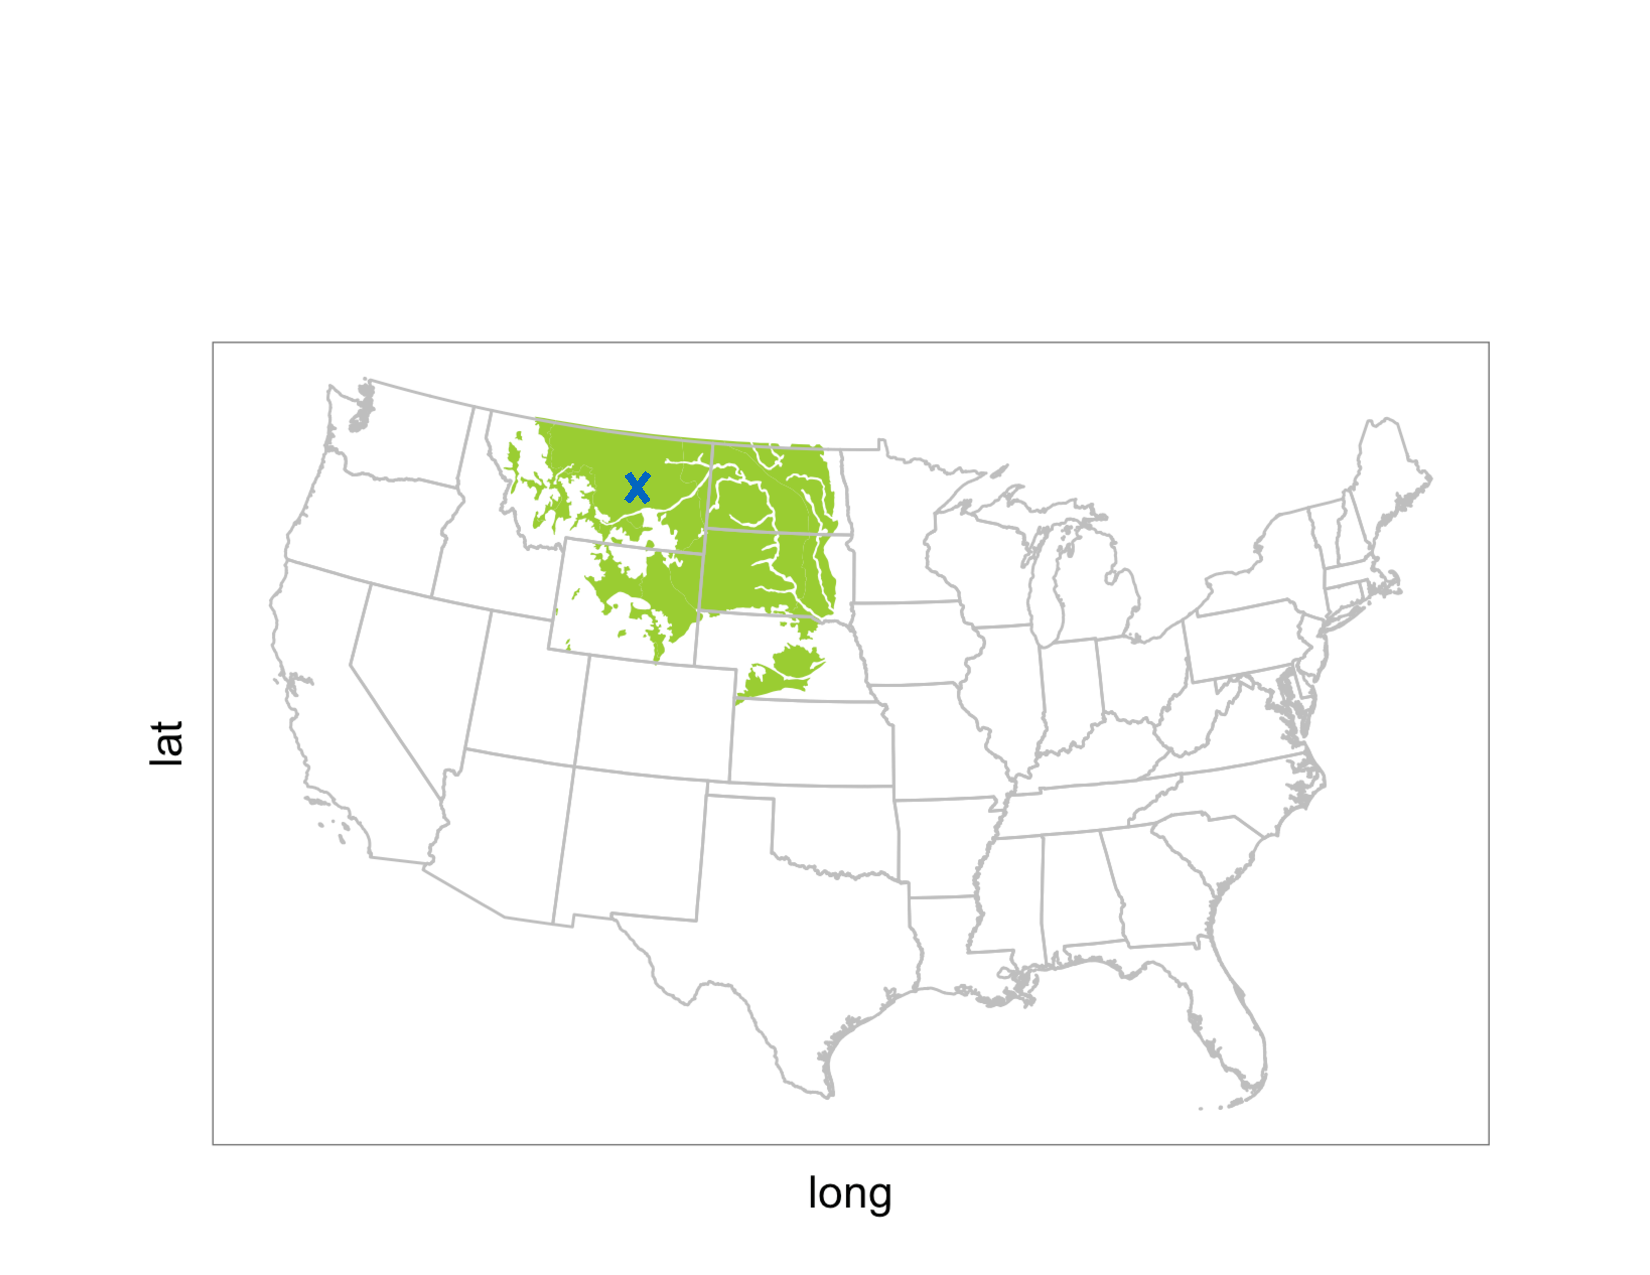
\includegraphics[height=2.8in]{./figures/managers_get.pdf}

\end{frame}

\begin{frame}{%
\protect\hypertarget{really-hard-work}{%
Really hard work}}

\includegraphics[width=\textwidth]{./figures/chart_measuring.jpg}

\end{frame}

\begin{frame}{%
\protect\hypertarget{do-we-need-demographic-data}{%
Do we need demographic data?}}

\centering

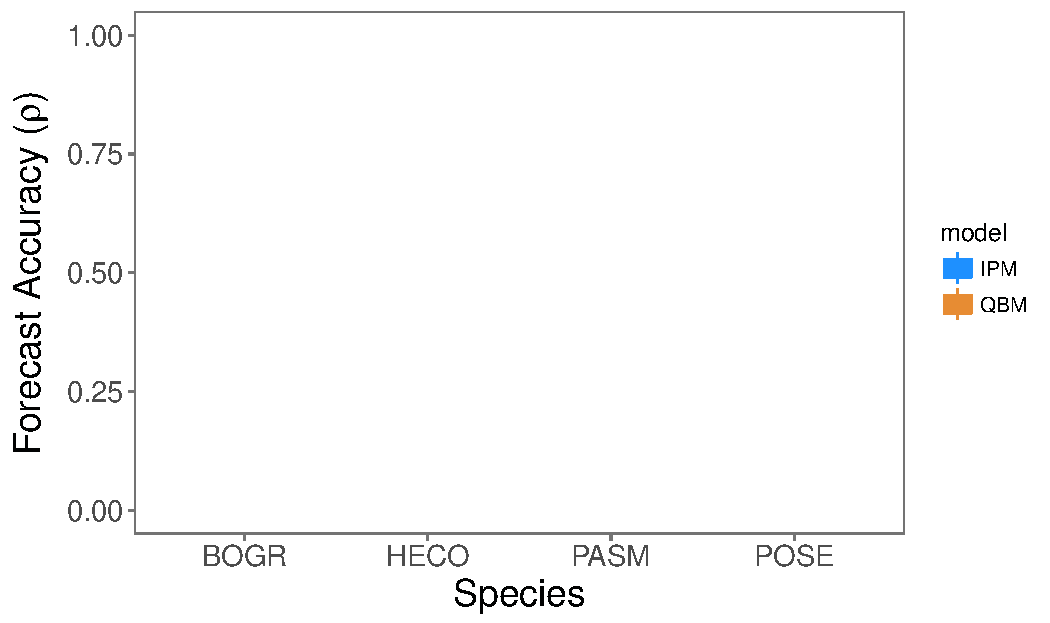
\includegraphics[height=2.5in]{./figures/mee_forecast_accuracy_empty.pdf}

\credit{Tredennick et al., 2017, \emph{Methods in Ecol. Evol.}}

\end{frame}

\begin{frame}{%
\protect\hypertarget{free-from-the-tyranny-of-demographic-data}{%
Free from the tyranny of demographic data!}}

\centering

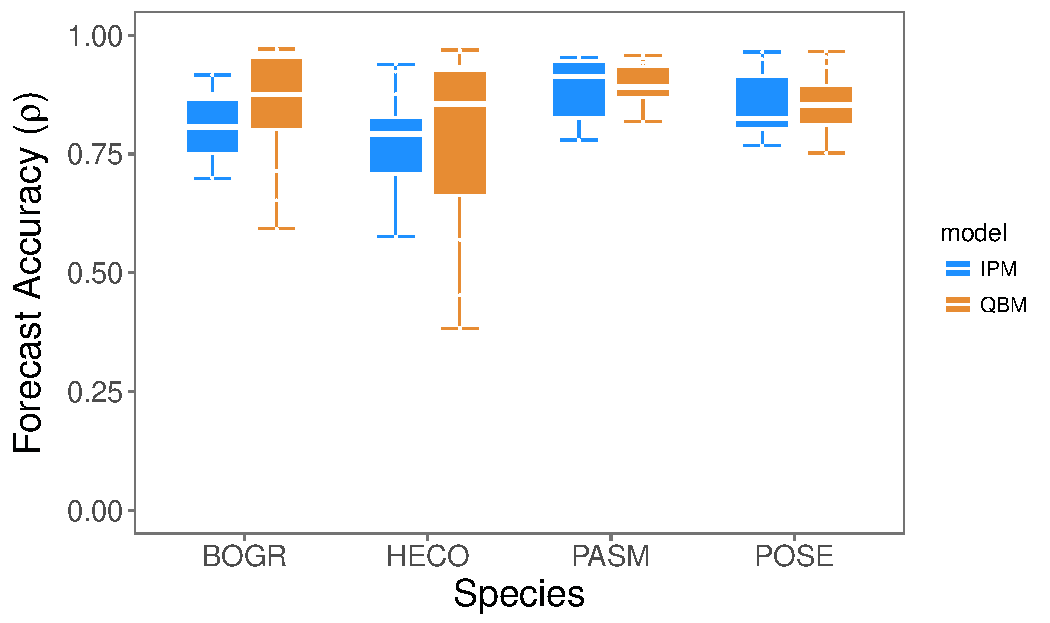
\includegraphics[height=2.5in]{./figures/mee_forecast_accuracy.pdf}

\credit{Tredennick et al., 2017, \emph{Methods in Ecol. Evol.}}

\end{frame}

\begin{frame}{%
\protect\hypertarget{lets-use-satellites}{%
Let’s use satellites}}

\centering

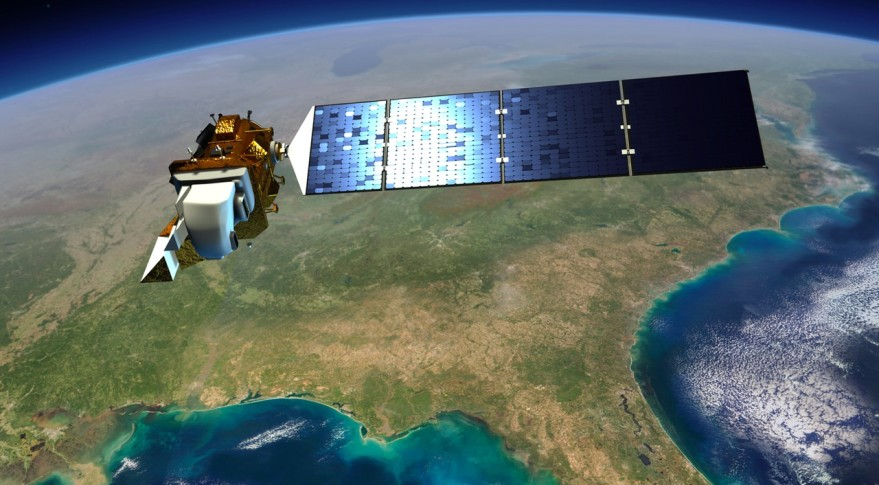
\includegraphics[height=2.7in]{./figures/landsat8.jpg}

\end{frame}

\begin{frame}{%
\protect\hypertarget{sagebrush-sea-in-wyoming}{%
Sagebrush sea in Wyoming}}

\centering

\includegraphics[height=2.5in]{./figures/sage_pic.pdf}

\end{frame}

\begin{frame}{%
\protect\hypertarget{study-area}{%
Study area}}

\centering

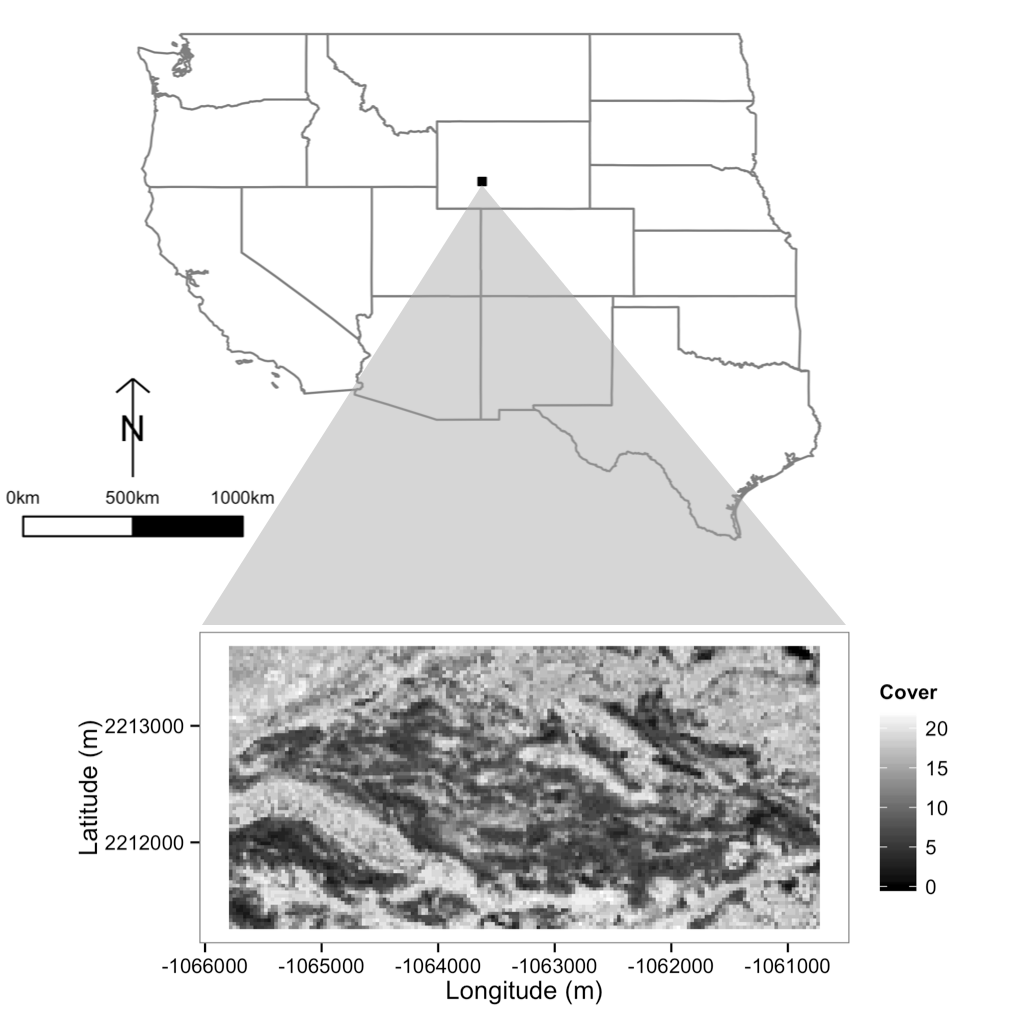
\includegraphics[height=2.8in]{./figures/studyarea_map.png}

\end{frame}

\begin{frame}{%
\protect\hypertarget{landsat-time-series}{%
Landsat time series}}

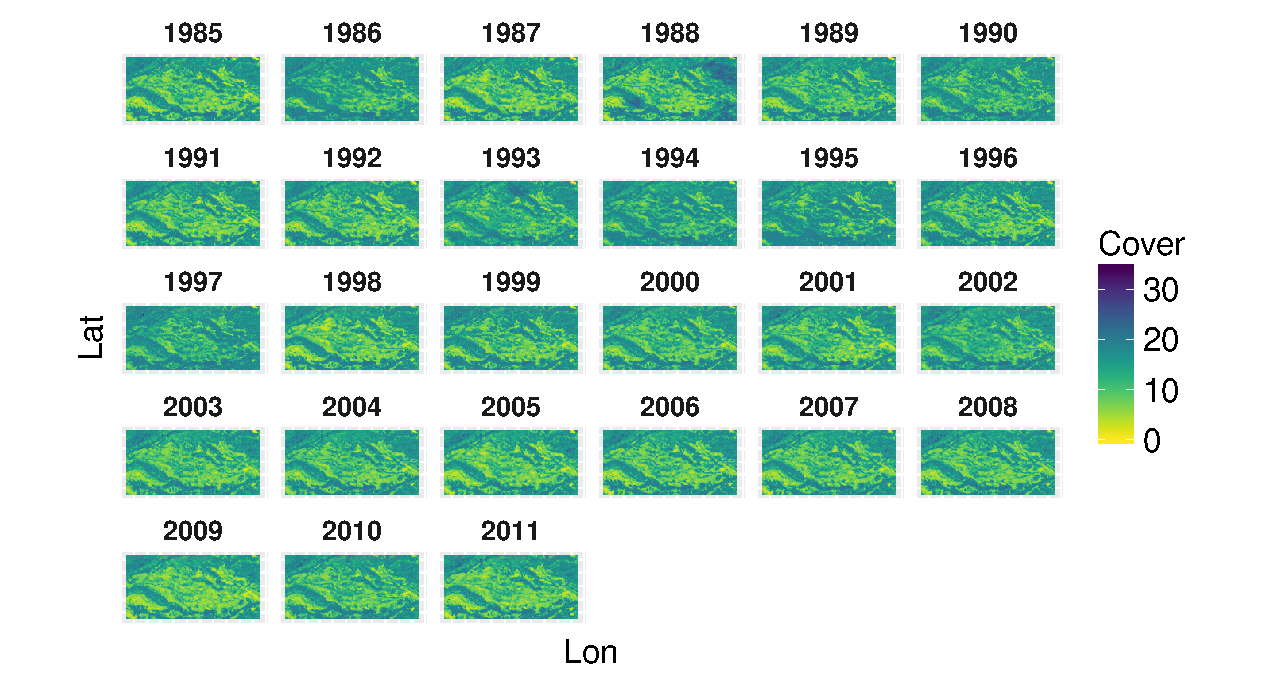
\includegraphics[height=2.8in]{./figures/all_years_percCover.pdf}

\end{frame}

\begin{frame}{%
\protect\hypertarget{dynamic-cover-model}{%
Dynamic cover model}}

\begin{align*}
y_{i,t} &\sim \text{Poisson}(\mu_{i,t}) \\
\text{log}(\mu_{i,t}) &= \underbrace{\beta_{0,t} + \beta_{1}y_{i,t-1}}_\text{temporal + dens. dep} + \underbrace{\textbf{x}_{t}'\boldsymbol{\gamma}}_\text{climate} + \underbrace{\eta_{i}}_\text{spatial}
\end{align*}

\end{frame}

\begin{frame}{%
\protect\hypertarget{dimension-reduction-for-spatial-effect}{%
Dimension reduction for spatial effect}}

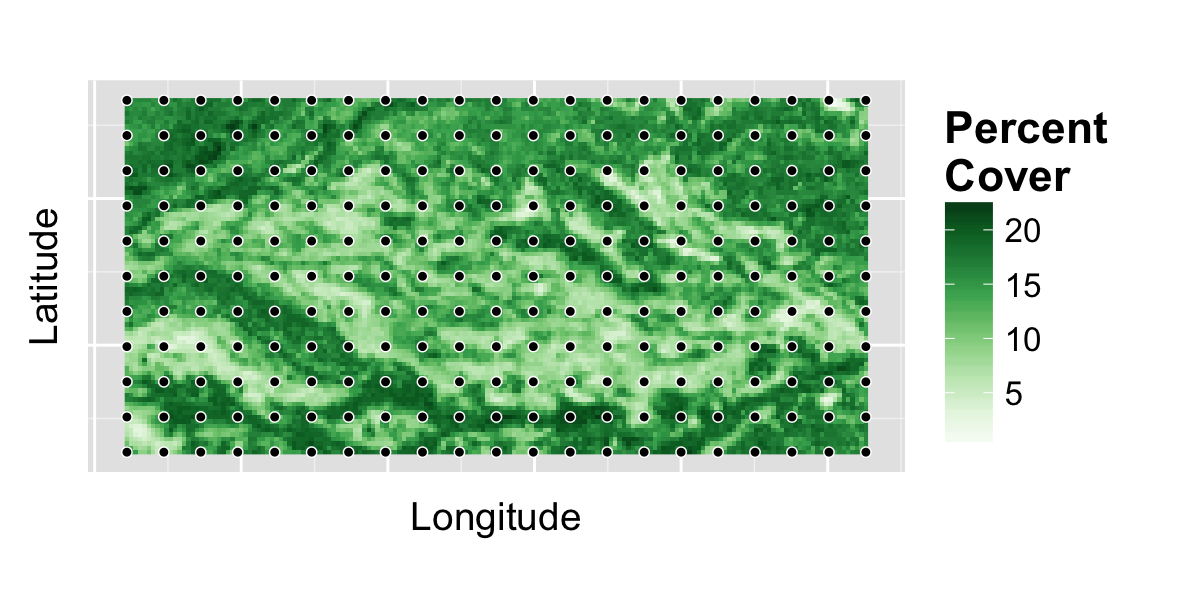
\includegraphics[width=\textwidth]{./figures/SAGE_Grid_wKnots_subset.png}

\end{frame}

\begin{frame}{%
\protect\hypertarget{dynamic-cover-model-1}{%
Dynamic cover model}}

\small

\begin{align*}
y_{i,t} &\sim \text{Poisson}(\mu_{i,t}) \\
\text{log}(\mu_{i,t}) &= \underbrace{\beta_{0,t} + \beta_{1}y_{i,t-1}}_\text{temporal + dens. dep} + \underbrace{\textbf{x}_{t}'\boldsymbol{\gamma}}_\text{climate} + \underbrace{\eta_{i}}_\text{spatial} \\
\boldsymbol{\eta} &\approx \textbf{K}\boldsymbol{\alpha}, \\
\textbf{K} &= \mathbf{w}_{s,m} / \sum_{s=1}^S \mathbf{w}_{s,m} \\
\mathbf{w}_{s,m} &= \text{exp}\left(-d_{s,m} / \sigma \right) \\
\alpha_{m} &\sim \text{Normal}(0,\sigma_{\eta}^2)
\end{align*}

\end{frame}

\begin{frame}{%
\protect\hypertarget{climate-covariates}{%
Climate covariates}}

\centering

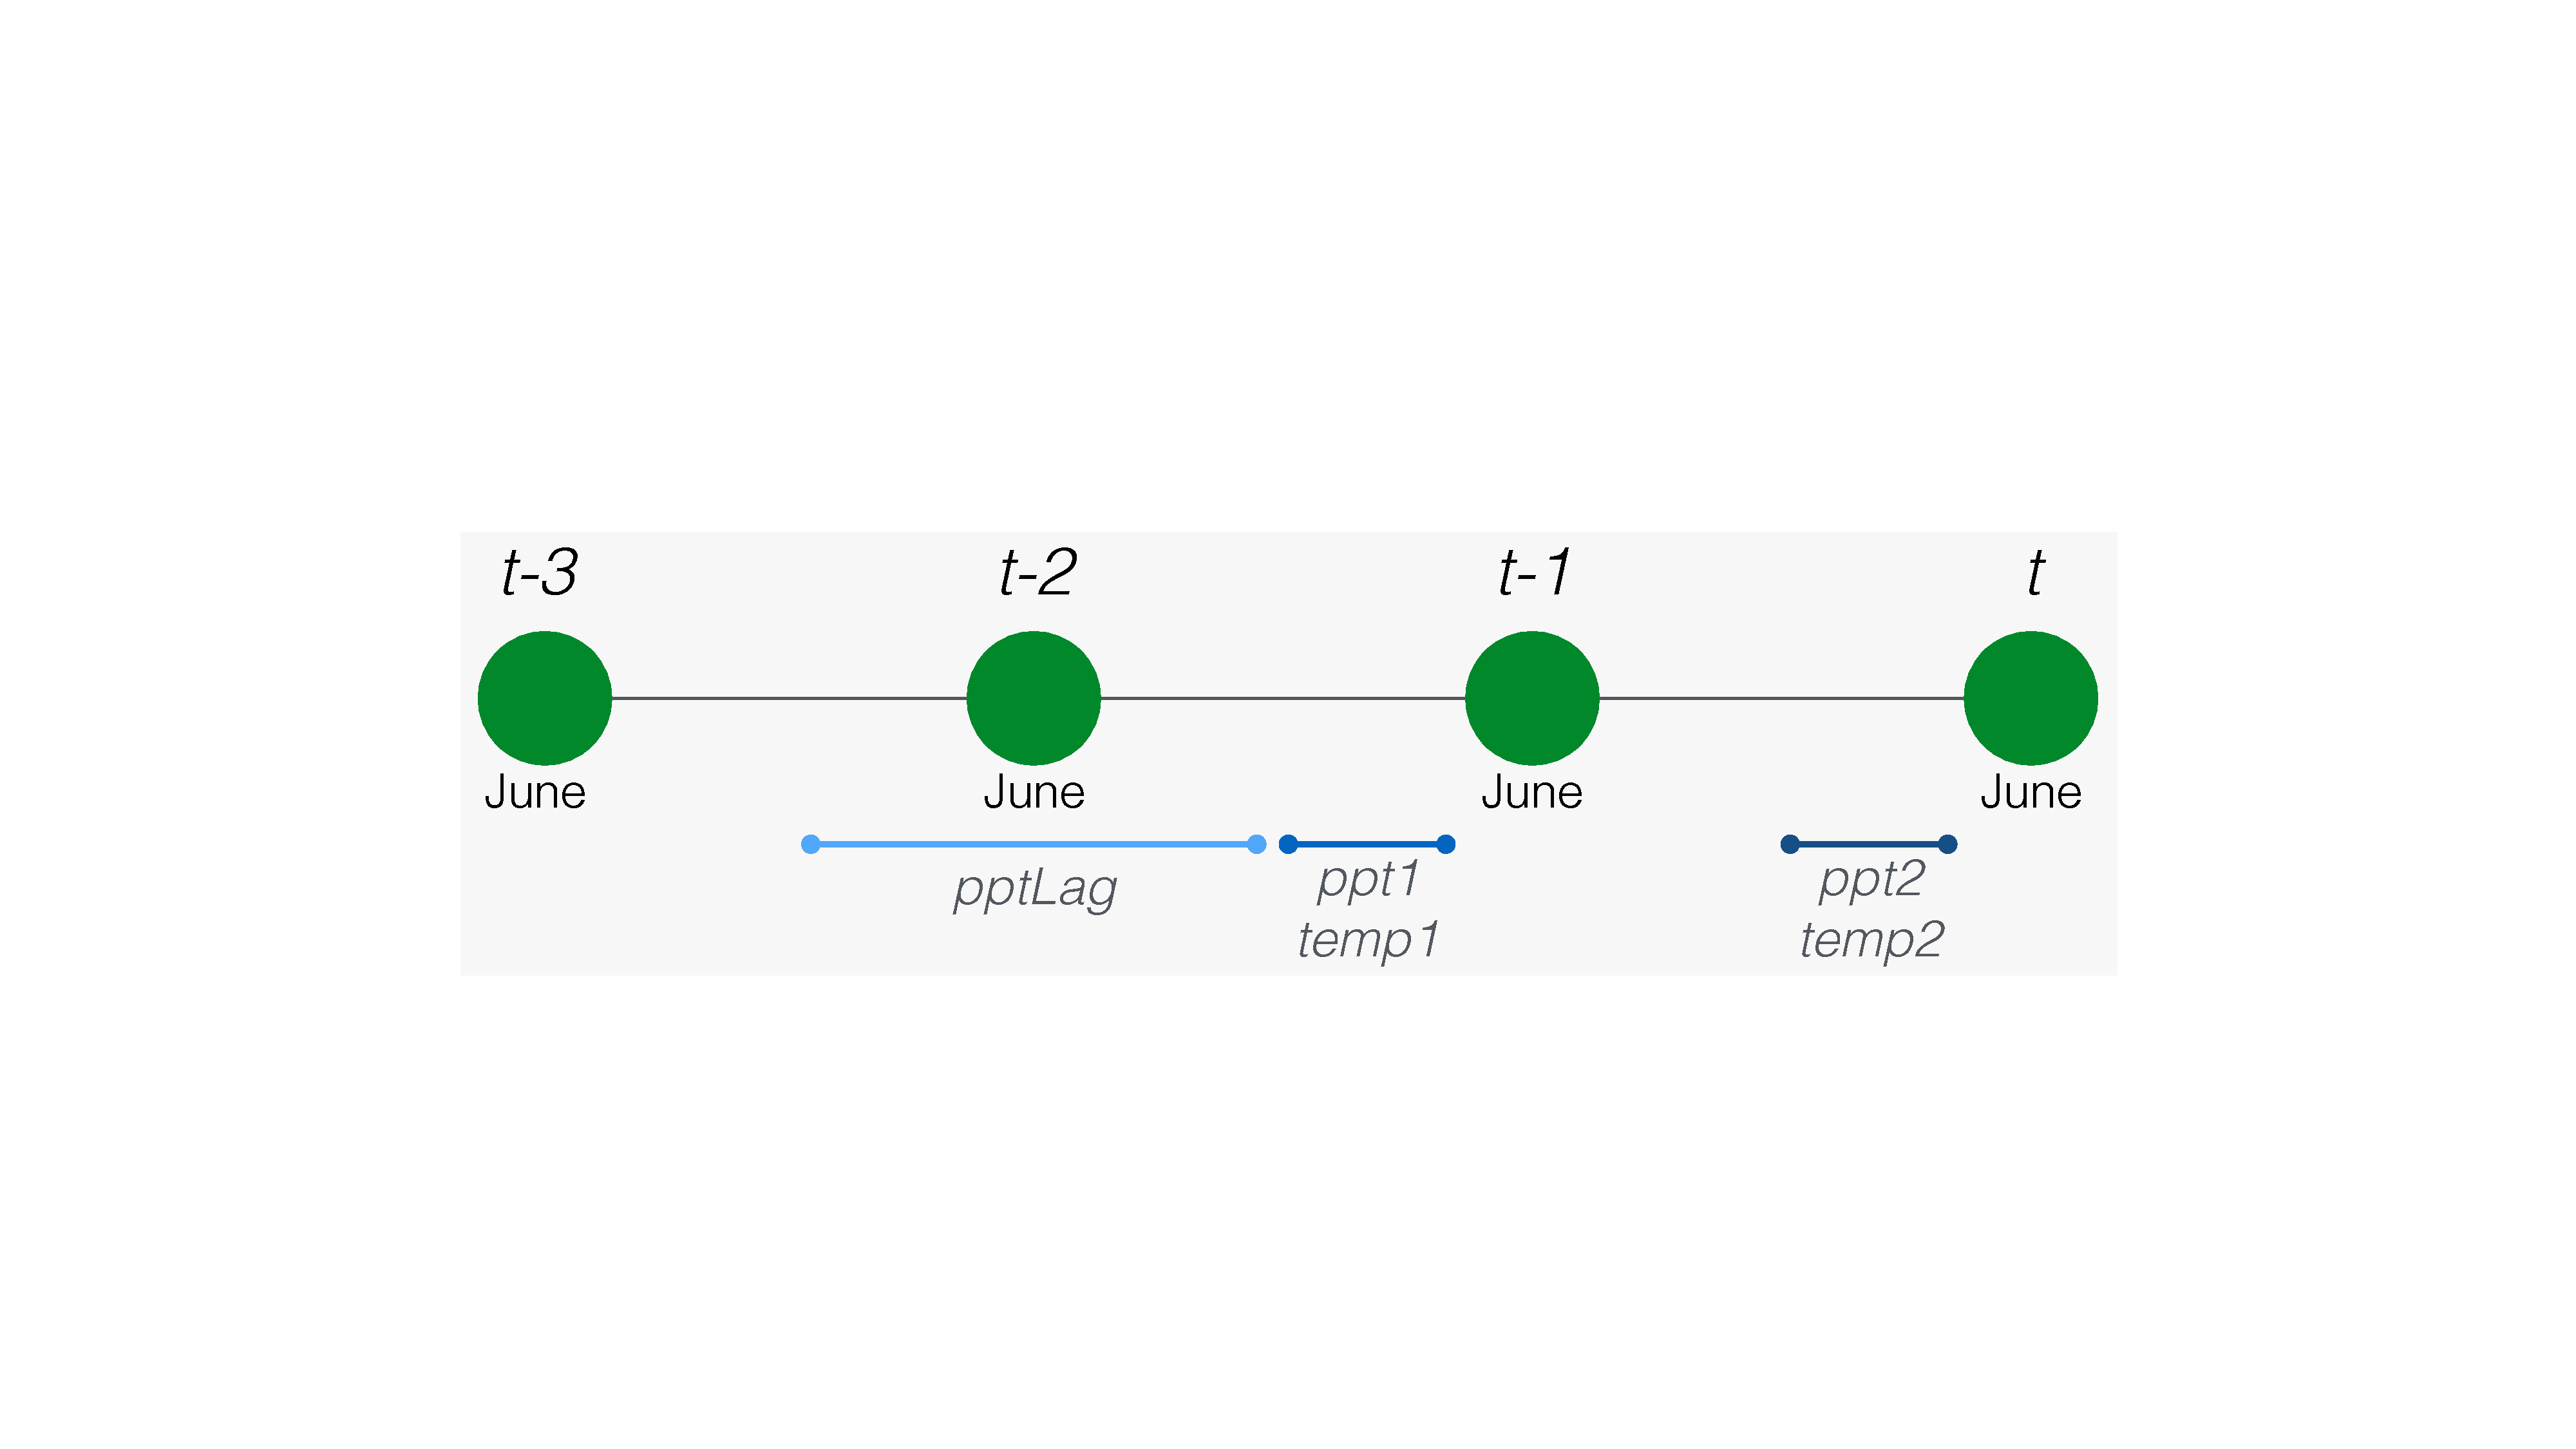
\includegraphics[width=\textwidth]{./figures/ipm_climate_effects.pdf}

\end{frame}

\begin{frame}{%
\protect\hypertarget{climate-effects}{%
Climate effects}}

\centering

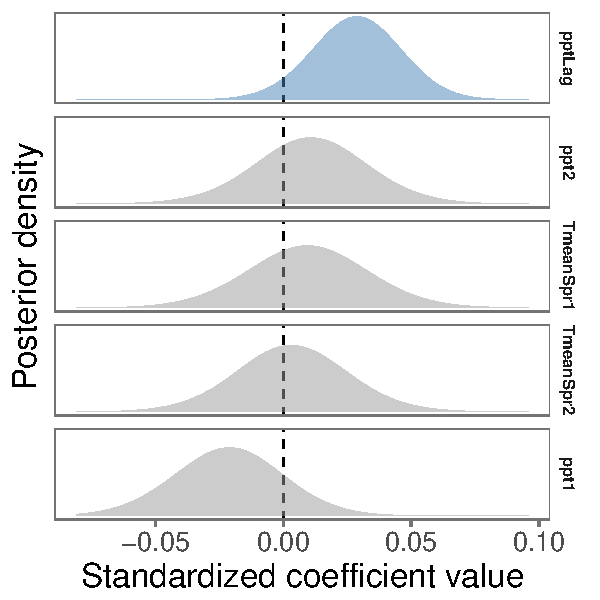
\includegraphics[height=2.7in]{./figures/post_climate_covariates.pdf}

\end{frame}

\begin{frame}{%
\protect\hypertarget{model-performance}

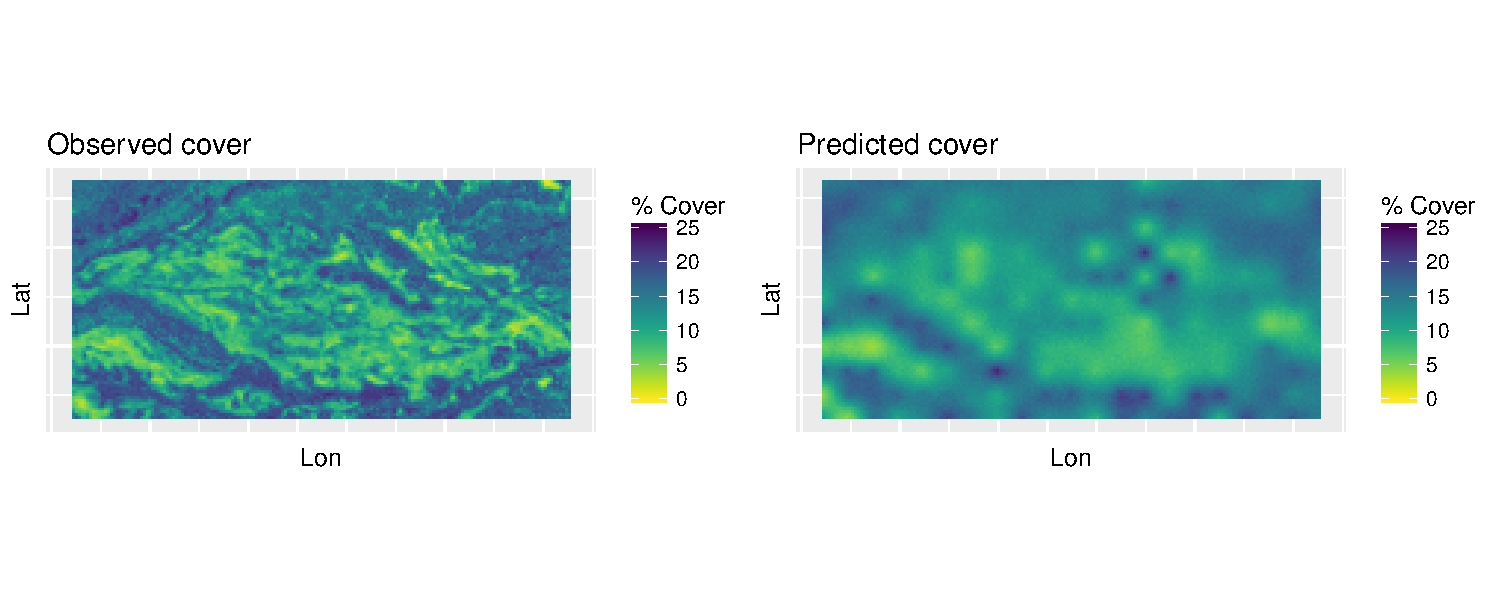
\includegraphics[width=\textwidth]{./figures/obs_predict_spatial_pres.pdf}

\credit{Tredennick et al., 2016, \emph{Ecosphere}}

\end{frame}

\begin{frame}{%
\protect\hypertarget{forecasts-under-climate-change-spatial}{%
Forecasts under climate change: spatial}}

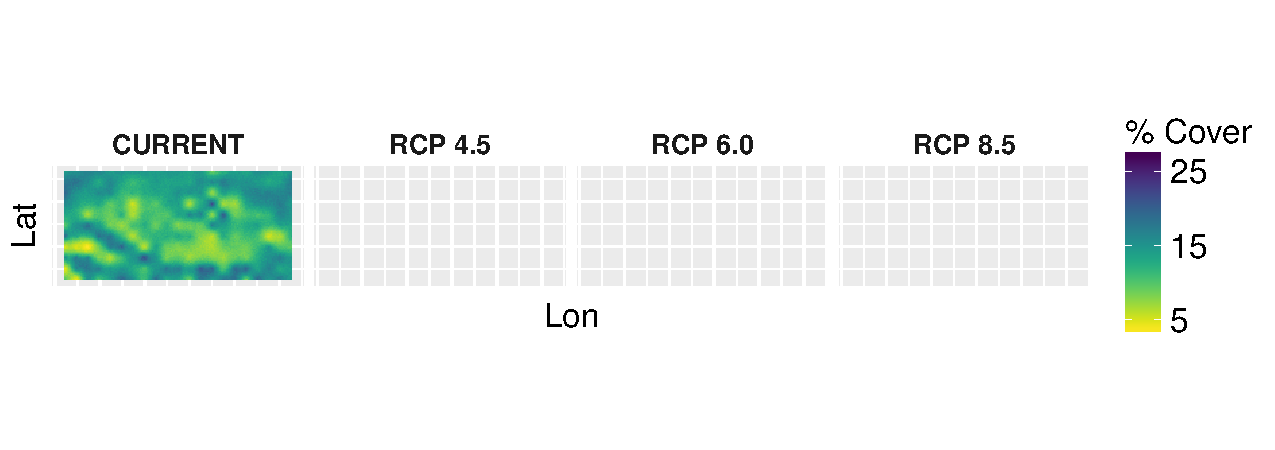
\includegraphics[width=\textwidth]{./figures/clim_change_mean_spatial_empty.pdf}

\credit{Tredennick et al., 2016, \emph{Ecosphere}}

\end{frame}

\begin{frame}{%
\protect\hypertarget{forecasts-under-climate-change-spatial-1}{%
Forecasts under climate change: spatial}}

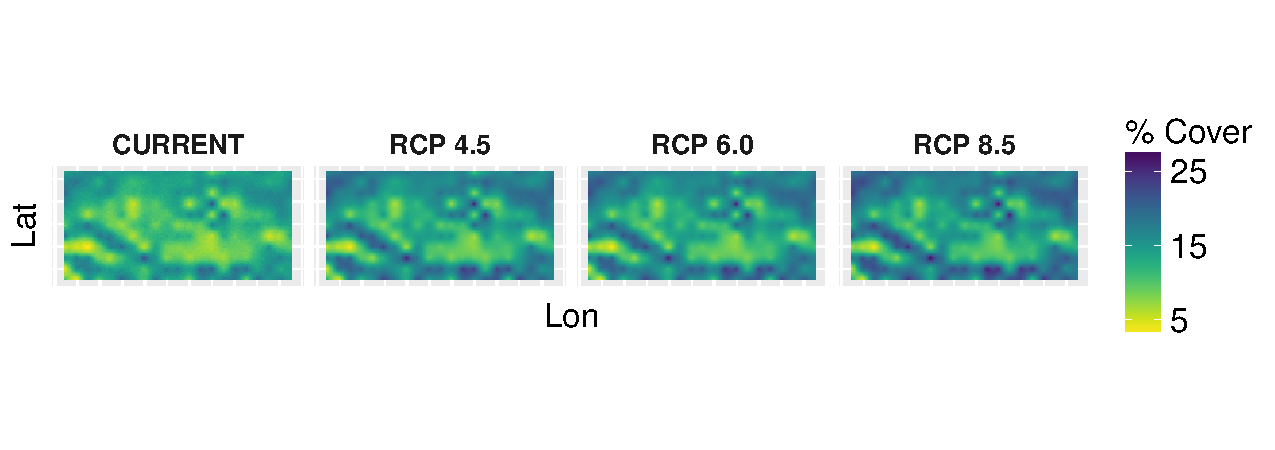
\includegraphics[width=\textwidth]{./figures/clim_change_mean_spatial.pdf}

\credit{Tredennick et al., 2016, \emph{Ecosphere}}

\end{frame}

\begin{frame}{%
\protect\hypertarget{forecasts-under-climate-change-temporal}{%
Forecasts under climate change: temporal}}

\centering

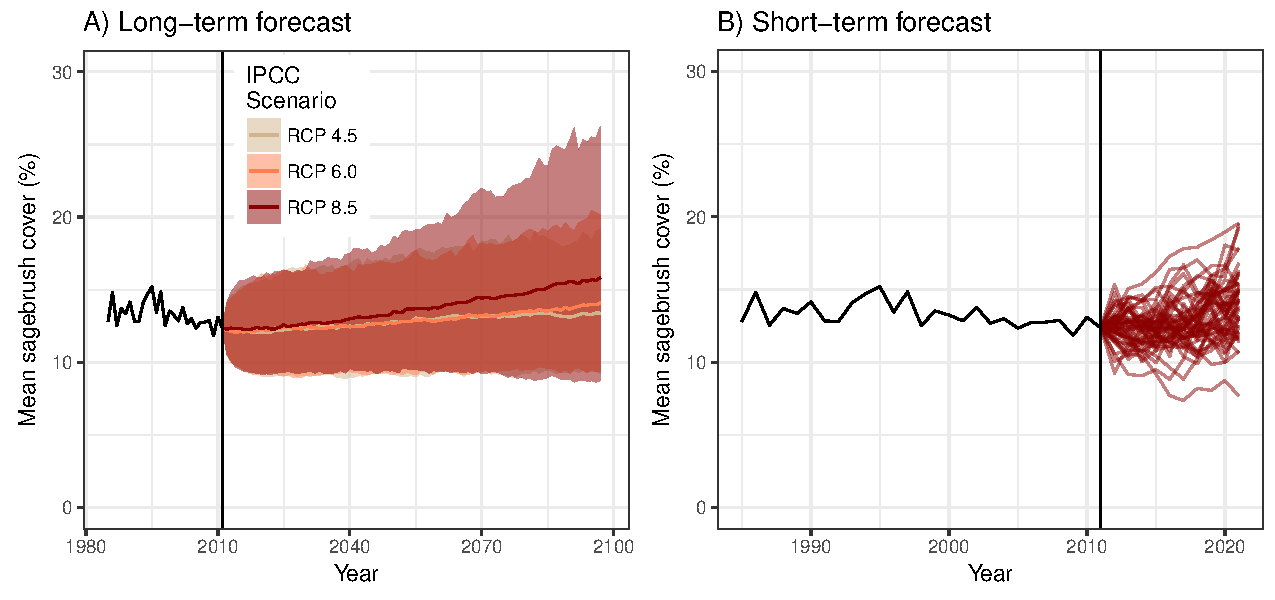
\includegraphics[height=2in]{./figures/temporal_forecasts_presentation.pdf}

\credit{Tredennick et al., 2016, \emph{Ecosphere}}

\end{frame}

\hypertarget{partitioning-forecast-uncertainty}{%
\section{Partitioning forecast
uncertainty}\label{partitioning-forecast-uncertainty}}

\begin{frame}{%
\protect\hypertarget{forecast-uncertainty-to-a-first-approximation}{%
Forecast uncertainty, to a first approximation}}

Forecast of state \(z\) at \(t+1\) from function \(q\):
\(q = f(z_t, x_t, \theta, \varepsilon_{t+1})\)

\small

\begin{align*}
\text{var}[y_{t+1}] \approx \underbrace{\left(\frac{\delta q}{\delta y} \right)^2}_{\text{stability}} 
               \underbrace{\vphantom{ \left(\frac{\delta q}{\delta y} \right)^2 } \text{var}[y_t]}_{\text{IC uncert.}} +
               \underbrace{\vphantom{ \left(\frac{\delta q}{\delta y} \right)^2 }\left(\frac{\delta f}{\delta x} \right)^2}_{\text{driver sens.}} 
               \underbrace{\vphantom{ \left(\frac{\delta q}{\delta y} \right)^2 } \text{var}[x_t]}_{\text{driver uncert.}} +
               \underbrace{\vphantom{ \left(\frac{\delta q}{\delta y} \right)^2 }\left(\frac{\delta f}{\delta \theta} \right)^2}_{\text{param sens.}}
               \underbrace{\vphantom{ \left(\frac{\delta q}{\delta y} \right)^2 } \text{var}[\theta]}_{\text{param. uncert.}} +
               \underbrace{\vphantom{ \left(\frac{\delta q}{\delta y} \right)^2 } \text{var}[\varepsilon_{t+1}]}_{\text{process error}}
\end{align*}

\credit{Dietze, 2017, \emph{Ecological Applications}}

\end{frame}

\begin{frame}{%
\protect\hypertarget{error-propagation}{%
Error propagation}}

For some function \(q\): \(q = f(x_1,x_2,\dots,x_n)\)

\begin{align*}
\sigma^2_q &= \left( \frac{\delta q}{\delta x_1} \sigma_{x_1} \right)^2 + \left( \frac{\delta q}{\delta x_2} \sigma_{x_2} \right)^2 + \cdots + \left( \frac{\delta q}{\delta x_n} \sigma_{x_n} \right)^2 \\
&= \sum^n_{i=1}\left( \frac{\delta q}{\delta x_i} \sigma_{x_i} \right)^2
\end{align*}

\credit{Ku, 1966, \emph{J. Res. National Bureau of Standards - C}}

\end{frame}

\begin{frame}{%
\protect\hypertarget{error-propagation-1}{%
Error propagation}}

\begin{align*}
\sigma^2_q &= \underbrace{\sum^n_{i=1}\left( \frac{\delta q}{\delta x_i} \sigma_{x_i} \right)^2}_{\text{variances}} + \alert{\underbrace{\sum^n_{i=1} \sum^n_{j(j \ne i)} 2 \sigma_{ij}\left( \frac{\delta q}{\delta x_i} \right)\left( \frac{\delta q}{\delta x_j} \right)}_{\text{covariances}}}
\end{align*}

\credit{Ku, 1966, \emph{J. Res. National Bureau of Standards - C}}

\end{frame}

\begin{frame}{%
\protect\hypertarget{can-we-ignore-covariances}{%
Can we ignore covariances?}}

\begin{align*}
z_{t+1} &= z_{t} \beta_0 + x_t \beta_1 + \varepsilon_{t+1}, \\
z_{t=1} &\sim \text{Normal}(z_0, \sigma^2_{\text{init.}}), \qquad \scriptstyle\text{initial conditions uncertainty} \\
\mathbf{\beta} &\sim \text{MVN}(0, \sigma^2_{\text{param.}} \mathbf{I}), \qquad \scriptstyle\text{parameter uncertainty} \\
\varepsilon_t &\sim \text{Normal}(0, \sigma^2_{\text{proc.}}) \qquad \scriptstyle\text{process uncertainty}
\end{align*}

\end{frame}

\begin{frame}{%
\protect\hypertarget{interaction-covariances-cannot-be-ignored}{%
Interaction (covariances) cannot be ignored}}

\centering

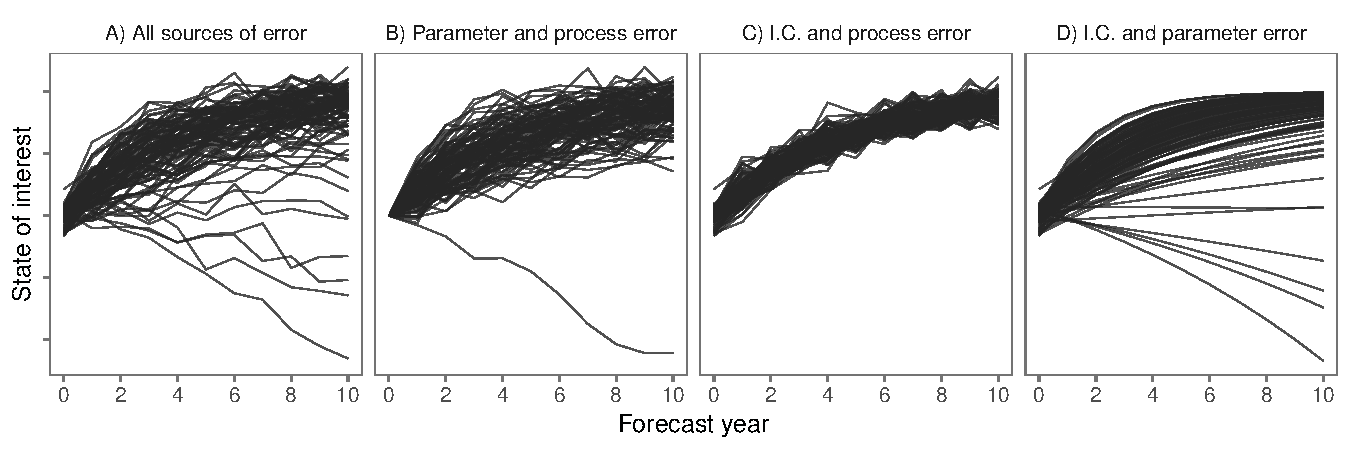
\includegraphics[width=\textwidth]{./figures/forecast_uncertainty_example.pdf}

\end{frame}

\begin{frame}{%
\protect\hypertarget{an-error-propogation-problem}{%
An \emph{inverse} error propogation problem}}

\small

\begin{align*}
\text{var}[y_{t+1}] \approx \underbrace{\left(\frac{\delta q}{\delta y} \right)^2}_{\text{stability}} 
               \underbrace{\vphantom{ \left(\frac{\delta q}{\delta y} \right)^2 } \text{var}[y_t]}_{\text{IC uncert.}} +
               \underbrace{\vphantom{ \left(\frac{\delta q}{\delta y} \right)^2 }\left(\frac{\delta f}{\delta x} \right)^2}_{\text{driver sens.}} 
               \underbrace{\vphantom{ \left(\frac{\delta q}{\delta y} \right)^2 } \text{var}[x_t]}_{\text{driver uncert.}} +
               \underbrace{\vphantom{ \left(\frac{\delta q}{\delta y} \right)^2 }\left(\frac{\delta f}{\delta \theta} \right)^2}_{\text{param sens.}}
               \underbrace{\vphantom{ \left(\frac{\delta q}{\delta y} \right)^2 } \text{var}[\theta]}_{\text{param. uncert.}} +
               \underbrace{\vphantom{ \left(\frac{\delta q}{\delta y} \right)^2 } \text{var}[\varepsilon_{t+1}]}_{\text{process error}}
\end{align*}

\end{frame}

\begin{frame}{%
\protect\hypertarget{hierarchical-bayesian-models-propagate-uncertainty-for-us}{%
Hierarchical Bayesian models propagate uncertainty for us}}

\begin{equation*}
\begin{aligned}[b]
\textbf{Data Model:} \quad y_t &\sim \left[y_t \;|\; z_t, \sigma^2_{\text{o}}\right], &t = 1,\dots,T, \\ 
\textbf{Process Models:} \quad z_t &\sim \left[z_t \;|\; \mu_t, \sigma^2_{\text{p}}\right],  \\ 
\mu_t &= g \left(z_{t-1},\textbf{x}'_t, \boldmath{\theta} \right), &t = 2,\dots,T, \\ 
\textbf{Parameter Models:} \quad \boldmath{\phi} &\sim \left[\boldmath{\theta},\sigma^2_{\text{p}},\sigma^2_{\text{o}},z_{t=1} \right]
\end{aligned}
\end{equation*}

\credit{Berliner, 1996, \emph{in} Maximum entropy and bayesian methods}

\end{frame}

\begin{frame}{%
\protect\hypertarget{the-forecast-distribution}{%
The Forecast distribution}}

\begin{equation*}
\begin{gathered}
\left[z_{T+1} | y_1,\dots,y_T \right] = \int \int \dots \int \left[z_{T+1} | z_T, \textbf{x}_T, \theta, \sigma^2_{\text{p}} \right] \\ \times \left[z_1,\dots,z_{T+1},\theta, \sigma^2_{\text{p}} | y_1,\dots,y_T \right] \alert{d \theta d \sigma^2_{\text{p}} d z_1 \dots d z_T d \textbf{x}_1 \dots d \textbf{x}_T}
\end{gathered}
\end{equation*}

\credit{Hobbs and Hooten, 2015, Bayesian Models: A Statistical Primer for Ecologists}

\end{frame}

\begin{frame}{%
\protect\hypertarget{the-forecast-distribution-via-mcmc}{%
The Forecast Distribution, via MCMC}}

We have:

\begin{itemize}
 \item $k = 1,\dots,K$ MCMC iterations
 \item $j = 1,\dots,J$ realizations of the covariate, resampled to match $K$
 \item Forecasts at times $T+q,\dots,T+Q$
\end{itemize}

\begin{equation*}
z_{T+q}^{(k)} \sim \left[z_{T+q} | g(z_{T+q-1}^{(k)}, \textbf{x}_{T+q}^{(j(k))},\boldmath{\theta}^{(k)}), \sigma^{2(k)}_{\text{p}} \right]
\end{equation*}

\end{frame}

\begin{frame}{%
\protect\hypertarget{partitioning-from-mcmc-samples}{%
\emph{Post hoc} partitioning from MCMC samples}}

\bf{Ignore initial conditions uncertainty}

\begin{equation*}
\alert{z_{T}^{(\ast)}} = E(z_{T} | y_1,\dots,y_T) \approx \frac{\sum^K_{k=1} z_{T}^{(k)}}{K}
\end{equation*}

\begin{equation*}
    z_{T+q} \sim 
\begin{cases}
    \left[z_{T+q} | g(z_{T+q-1}^{(k)}, \textbf{x}_T^{(j(k))}, \boldmath{\theta}^{(k)}), \sigma^{2(k)}_{\text{p}} \right], &q>1 \\
    \left[z_{T+q} | g(\alert{z_{T}^{(\ast)}}, \textbf{x}_T^{(j(k))}, \boldmath{\theta}^{(k)}), \sigma^{2(k)}_{\text{p}} \right], &q=1.
\end{cases}
\end{equation*}

\end{frame}

\begin{frame}{%
\protect\hypertarget{partitioning-from-mcmc-samples-1}{%
\emph{Post hoc} partitioning from MCMC samples}}

\bf{ONLY initial conditions uncertainty}

\begin{align*}
\textbf{z}^{(I)}_{T+q} &= \textbf{z}_{T+q}^{(I,\overline{PA},\overline{D},\overline{PS})} \\
\textbf{z}^{(I)}_{T+q} &\approx \left[z_{T+q} \; | \; g(z_{T+q-1}^{(k)}, \alert{\textbf{x}^{(\ast)}_T, \boldmath{\theta}^{(\ast)}}), \alert{0} \right]
\end{align*}

\end{frame}

\begin{frame}{%
\protect\hypertarget{partitioning-from-mcmc-samples-2}{%
\emph{Post hoc} partitioning from MCMC samples}}

\begin{align*}
\textbf{z}^{(I)}_{T+q} &= \textbf{z}_{T+q}^{(I,\overline{PA},\overline{D},\overline{PS})} \\
\textbf{z}^{(I)}_{T+q} &\approx \left[z_{T+q} \; | \; g(z_{T+q-1}^{(k)}, \alert{\textbf{x}^{(\ast)}_T, \boldmath{\theta}^{(\ast)}}), \alert{0} \right] \\
V^{(I)}_{T+q} &= \text{var}(\textbf{z}^{(I)}_{T+q})
\end{align*}

\end{frame}

\begin{frame}{%
\protect\hypertarget{partitioning-from-mcmc-samples-3}{%
\emph{Post hoc} partitioning from MCMC samples}}

\begin{longtable}[]{@{}ll@{}}
\toprule
\begin{minipage}[b]{0.29\columnwidth}\raggedright
Source of Uncertainty\strut
\end{minipage} & \begin{minipage}[b]{0.25\columnwidth}\raggedright
Notation\strut
\end{minipage}\tabularnewline
\midrule
\endhead
\begin{minipage}[t]{0.29\columnwidth}\raggedright
Initial conditions\strut
\end{minipage} & \begin{minipage}[t]{0.25\columnwidth}\raggedright
\(V^{(I) \ } = V^{(I,\overline{PA},\overline{D},\overline{PS})}\)\strut
\end{minipage}\tabularnewline
\begin{minipage}[t]{0.29\columnwidth}\raggedright
Parameter uncertainty\strut
\end{minipage} & \begin{minipage}[t]{0.25\columnwidth}\raggedright
\(V^{(PA)} = V^{(\overline{I},PA,\overline{D},\overline{PS})}\)\strut
\end{minipage}\tabularnewline
\begin{minipage}[t]{0.29\columnwidth}\raggedright
Driver uncertainty\strut
\end{minipage} & \begin{minipage}[t]{0.25\columnwidth}\raggedright
\(V^{(D) \ } = V^{(\overline{I},\overline{PA},D,\overline{PS})}\)\strut
\end{minipage}\tabularnewline
\begin{minipage}[t]{0.29\columnwidth}\raggedright
Process uncertainty\strut
\end{minipage} & \begin{minipage}[t]{0.25\columnwidth}\raggedright
\(V^{(PS)}=V^{(\overline{I},\overline{PA},\overline{D},PS)}\)\strut
\end{minipage}\tabularnewline
\bottomrule
\end{longtable}

\end{frame}

\begin{frame}{%
\protect\hypertarget{partition-forecast-uncertainty-anova}{%
Partition Forecast Uncertainty: ANOVA}}

\begin{equation*}
\begin{aligned}[b]
V_{T+q}^{(F)} = \ &V_{T+q}^{(I)} + V_{T+q}^{(PA)} + V_{T+q}^{(D)} + V_{T+q}^{(PS)}
\end{aligned}
\end{equation*}

\end{frame}

\begin{frame}{%
\protect\hypertarget{partition-forecast-uncertainty-anova-1}{%
Partition Forecast Uncertainty: ANOVA}}

\begin{equation*}
\begin{aligned}[b]
V_{T+q}^{(F)} = \ &V_{T+q}^{(I)} + V_{T+q}^{(PA)} + V_{T+q}^{(D)} + V_{T+q}^{(PS)} \\
&+ \varepsilon_{T+q}^{(I,PA)} + \varepsilon_{T+q}^{(I,D)} + \varepsilon_{T+q}^{(I,PS)} + \varepsilon_{T+q}^{(PA,PS)} + \varepsilon_{T+q}^{(PA,D)} + \varepsilon_{T+q}^{(D,PS)} \\
&+ \varepsilon_{T+q}^{(I,PA,D)} + \varepsilon_{T+q}^{(I,PA,PS)} + \varepsilon_{T+q}^{(I,D,PS)} + \varepsilon_{T+q}^{(PA,D,PS)} \\
&+ \varepsilon_{T+q}^{(I,PA,D,PS)}
\end{aligned}
\end{equation*}

\end{frame}

\begin{frame}{%
\protect\hypertarget{partition-forecast-uncertainty-anova-2}{%
Partition Forecast Uncertainty: ANOVA}}

Example where forecast is influenced by initial conditions (\(I\)) and
parameter uncertainty (\(PA\)):

\begin{equation*}
V^{(F)}_{T+q} = V^{(I)}_{T+q} + V^{(PA)}_{T+q} + \alert{\varepsilon_{T+q}^{(I,PA)}}
\end{equation*}

so,

\begin{equation*}
\alert{\varepsilon_{T+q}^{(I,PA)}} = V^{(F)}_{T+q} - \left[ V^{(I)}_{T+q} + V^{(PA)}_{T+q} \right]
\end{equation*}

\end{frame}

\begin{frame}{%
\protect\hypertarget{return-to-example-of-ar1-process}{%
Return to example of AR(1) process}}

\centering

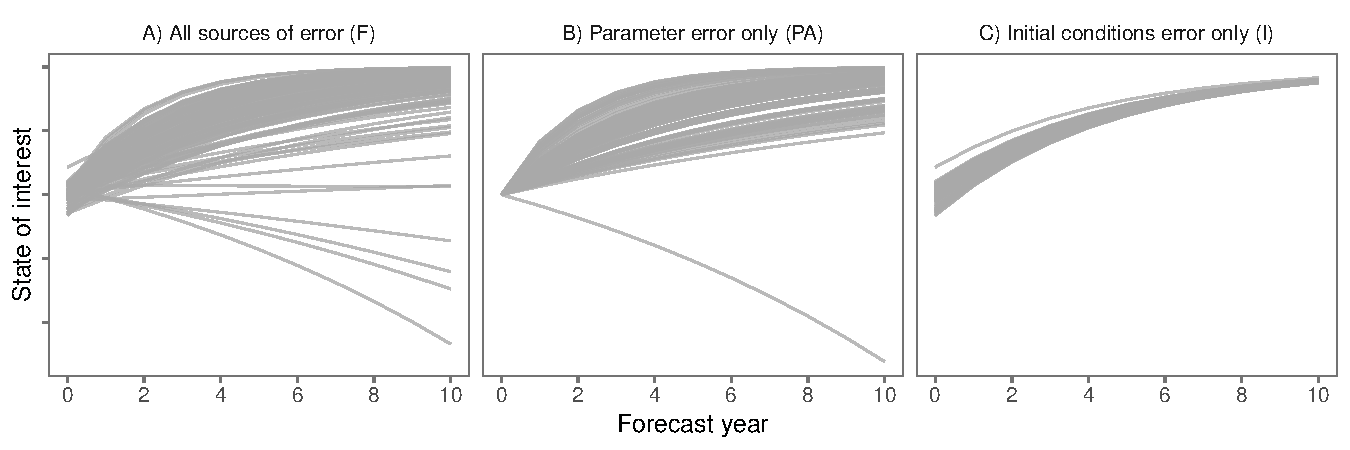
\includegraphics[width=\textwidth]{./figures/forecast_uncertainty_example2.pdf}

\end{frame}

\begin{frame}{%
\protect\hypertarget{partitioned-forecast-variance-over-time}{%
Partitioned forecast variance over time}}

\centering

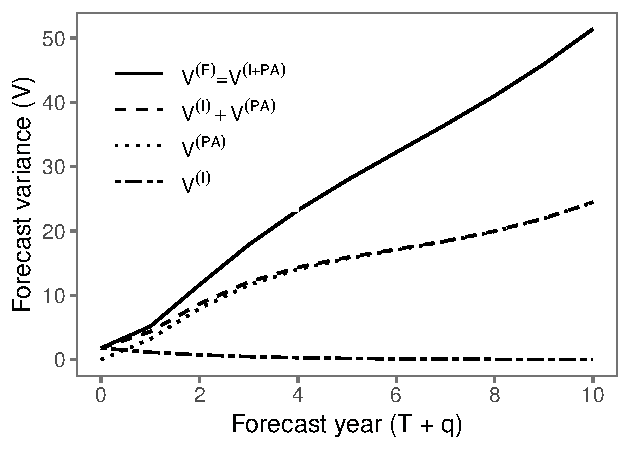
\includegraphics[height=2.5in]{./figures/example_interaction_effect_norib.pdf}

\end{frame}

\begin{frame}{%
\protect\hypertarget{partitioned-forecast-variance-over-time-1}{%
Partitioned forecast variance over time}}

\centering

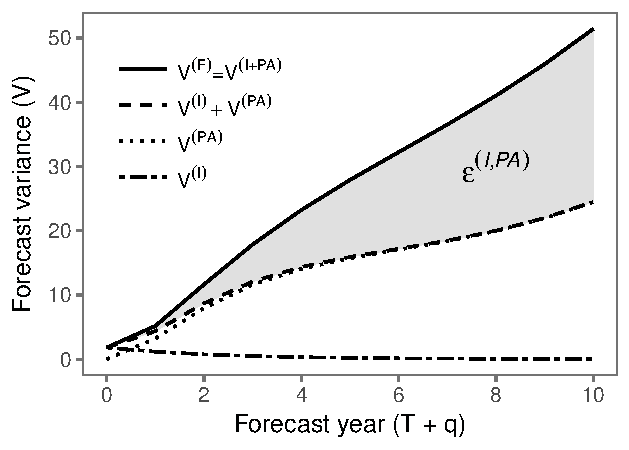
\includegraphics[height=2.5in]{./figures/example_interaction_effect.pdf}

\end{frame}

\hypertarget{conclusions}{%
\section{Conclusions}\label{conclusions}}

\begin{frame}{%
\protect\hypertarget{conclusions-1}{%
Conclusions}}

\begin{enumerate}
[1.]
\tightlist
\item
  Partition uncertainty to \alert{advance ecological forecasting} – how
  do we get better?
\item
  Partition uncertainty to \alert{advance scientific progress} – what
  don’t we know?
\item
  Hierarchical Bayesian models ideally suited for partitioning
  uncertainty because they allow us to fully specify the inclusion of
  uncertainty.
\item
  Proof of concept – formal treatment in the works.
\end{enumerate}

\end{frame}

\begin{frame}[plain]
  \begin{picture}(0,0)
    \put(-28.5,-175){%
      \pgfuseimage{titlebackground}
    }
  \end{picture}
\end{frame}

\end{document}
